\documentclass[11pt]{article}

\usepackage[utf8]{inputenc}
\usepackage[T1]{fontenc}
\usepackage[spanish]{babel}
\usepackage{lmodern}
\usepackage[margin=2.5cm]{geometry}
\usepackage{graphicx}
\usepackage{booktabs}
\usepackage{amsmath}
\usepackage{listings}
\usepackage{xcolor}
\usepackage{float}
\usepackage{caption}
\usepackage{url}
\usepackage[hidelinks]{hyperref}

\lstset{
  language=C++,
  basicstyle=\ttfamily\small,
  keywordstyle=\color{blue}\bfseries,
  commentstyle=\color{gray}\itshape,
  backgroundcolor=\color{gray!8},
  numbers=left,
  numberstyle=\tiny,
  breaklines=true,
  showstringspaces=false,
  captionpos=b
}
\renewcommand{\lstlistingname}{Código}

\title{Laboratorio 2\\
Evaluación del desempeño de algoritmos y comportamiento de la memoria caché}
\author{[Nombre del estudiante]\\Universidad Nacional de San Agustín de Arequipa}
\date{\today}

\begin{document}
\maketitle

%------------------------------------------------------------
\section{Introducción}

La complejidad de un algoritmo cuenta cuántas operaciones realiza, pero no
dice nada sobre dónde están los datos que usa. En un computador real, leer
un dato que está en la caché L1 es mucho más rápido que traerlo de la
memoria principal. Por eso dos programas con la misma complejidad pueden
tardar tiempos muy diferentes.

El objetivo de este trabajo es comprobar esto de forma experimental. Se
comparan algoritmos que tienen la misma complejidad pero distinto patrón de
acceso a memoria: los dos pares de bucles anidados del libro de Pacheco, la
multiplicación clásica de matrices y la multiplicación por bloques. Los
programas se ejecutaron en dos equipos con distinto tamaño de caché, se
midieron sus tiempos y se analizaron con Valgrind (Cachegrind) para contar
los fallos de caché.

Los resultados muestran que recorrer una matriz por columnas puede ser hasta
20 veces más lento que por filas, y que la multiplicación por bloques puede
ser hasta 10,9 veces más rápida que la clásica, aunque en todos los casos el
número de operaciones es el mismo. La diferencia se explica por los fallos
de caché.

%------------------------------------------------------------
\section{Entorno de pruebas}

Las pruebas se hicieron en dos equipos. En ambos se usó una máquina virtual
con Lubuntu dentro de VMware (cuadro~\ref{tab:entorno}).

\begin{table}[H]
\centering
\caption{Equipos utilizados.}
\label{tab:entorno}
\begin{tabular}{lll}
\toprule
 & \textbf{Laptop} & \textbf{PC} \\
\midrule
Procesador & Intel i5-3230M & Intel i5-10400 \\
Núcleos / hilos & 2 / 4 & 6 / 12 \\
Caché L1 datos & 32 KB & 32 KB \\
Caché L2 & 256 KB & 256 KB \\
Caché L3 & 3 MB & 12 MB \\
\midrule
Máquina virtual & \multicolumn{2}{c}{Lubuntu 16.04 (32 bits), 4 vCPU, 2 GB RAM} \\
Compilador & \multicolumn{2}{c}{g++ 5.4.0, opciones \texttt{-std=c++14 -O2 -g}} \\
Valgrind & \multicolumn{2}{c}{3.11.0} \\
\bottomrule
\end{tabular}
\end{table}

\textbf{Forma de medir:} el tiempo se mide con
\texttt{std::chrono::high\_resolution\_clock}, solo alrededor de los bucles
(la inicialización de las matrices queda fuera). Cada caso se ejecutó 3
veces y se reporta el promedio. Las matrices se guardan en un
\texttt{vector} de tamaño $n \times n$, fila por fila, de modo que el
elemento $(i,j)$ está en la posición \texttt{i*n + j}.

\textbf{Limitaciones:} las mediciones se hicieron dentro de máquinas
virtuales y sin fijar el proceso a un núcleo, por lo que pueden tener algo
de ruido. En la PC, las otras tres máquinas virtuales del clúster estaban
encendidas pero sin ejecutar nada. Los tiempos menores a unos pocos
milisegundos son los más sensibles a este ruido.

%------------------------------------------------------------
\section{Análisis de bucles anidados}

\subsection{Código}

Se implementaron los dos pares de bucles del capítulo 2 de
Pacheco~\cite{pacheco}, que calculan $y = Ax$ (programa
\texttt{bucles.cpp}):

\begin{lstlisting}[caption={Primer par: recorre $A$ por filas.}]
for (int i = 0; i < MAX; i++)
    for (int j = 0; j < MAX; j++)
        y[i] += A[i * MAX + j] * x[j];
\end{lstlisting}

\begin{lstlisting}[caption={Segundo par: recorre $A$ por columnas.}]
for (int j = 0; j < MAX; j++)
    for (int i = 0; i < MAX; i++)
        y[i] += A[i * MAX + j] * x[j];
\end{lstlisting}

\subsection{Número de iteraciones y complejidad}

En los dos casos el bucle externo da $\mathit{MAX}$ vueltas y el interno otras
$\mathit{MAX}$, así que el cuerpo se ejecuta
\[
\sum_{i=0}^{\mathit{MAX}-1} \sum_{j=0}^{\mathit{MAX}-1} 1 = \mathit{MAX}^2
\]
veces. Como el cuerpo hace un número fijo de operaciones, los dos pares son
$O(\mathit{MAX}^2)$. Solo cambia el orden en que se recorre la matriz.

\subsection{Resultados}

\begin{table}[H]
\centering
\caption{Tiempo (s) de los dos pares de bucles y cuántas veces es más lento
el recorrido por columnas.}
\label{tab:bucles}
\small
\begin{tabular}{rrr|rrr|rrr}
\toprule
 & & & \multicolumn{3}{c|}{\textbf{Laptop}} & \multicolumn{3}{c}{\textbf{PC}} \\
MAX & Iteraciones & Tam. $A$ & Filas & Columnas & Veces & Filas & Columnas & Veces \\
\midrule
500  & 250\,000    & 1,9 MB & 0,00029 & 0,00060 & 2,0  & 0,00030 & 0,00030 & 1,0 \\
1000 & 1\,000\,000  & 7,6 MB & 0,00162 & 0,01881 & 11,6 & 0,00130 & 0,00308 & 2,4 \\
2000 & 4\,000\,000  & 30,5 MB & 0,00767 & 0,08411 & 11,0 & 0,00505 & 0,03467 & 6,9 \\
3000 & 9\,000\,000  & 68,7 MB & 0,01183 & 0,20526 & 17,4 & 0,01103 & 0,08723 & 7,9 \\
4000 & 16\,000\,000 & 122 MB & 0,01994 & 0,40370 & 20,2 & 0,01955 & 0,17042 & 8,7 \\
\bottomrule
\end{tabular}
\end{table}

\begin{figure}[H]
\centering
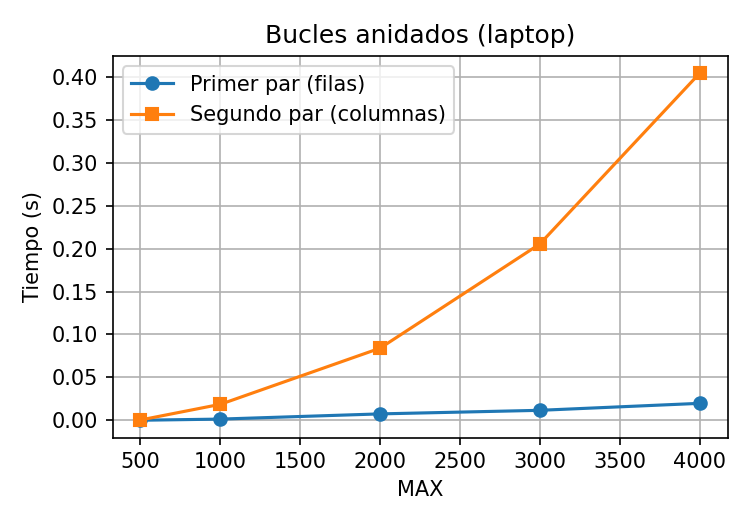
\includegraphics[width=0.48\textwidth]{../graficas/laptop_bucles.png}
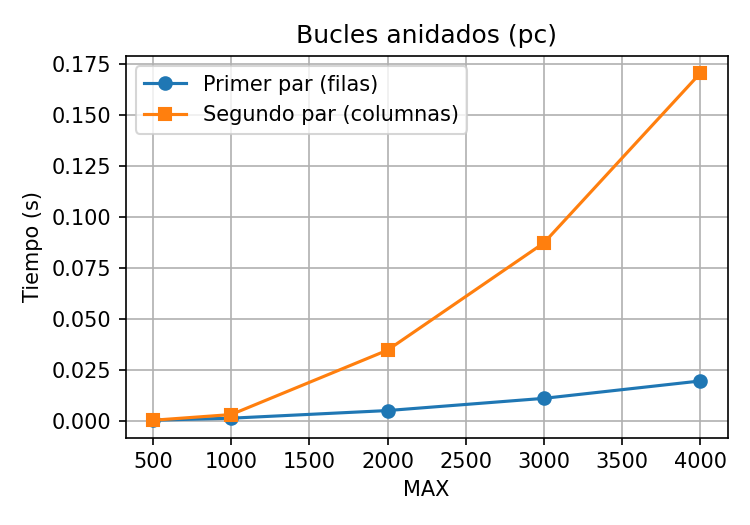
\includegraphics[width=0.48\textwidth]{../graficas/pc_bucles.png}
\caption{Tiempo de los dos pares de bucles en la laptop (izquierda) y en la PC (derecha).}
\label{fig:bucles}
\end{figure}

\subsection{Análisis}

Aunque los dos pares hacen exactamente las mismas iteraciones, el recorrido
por columnas es más lento, y la diferencia crece con $\mathit{MAX}$: en la laptop
llega a ser \textbf{20 veces} más lento y en la PC \textbf{8,7 veces}.

La razón es que la matriz está guardada por filas. Cuando se recorre por
filas, \texttt{A[i*MAX+j]} y \texttt{A[i*MAX+j+1]} están juntos en memoria,
y cada vez que la caché carga una línea de 64 bytes trae 8 elementos que se
van a usar enseguida. Cuando se recorre por columnas, cada acceso salta
$\mathit{MAX}$ posiciones, así que casi cada acceso cae en una línea distinta
y se produce un fallo de caché.

También se ve la influencia del tamaño de la caché L3. En la laptop (L3 de
3 MB) la diferencia salta de 2 a 11,6 veces entre $\mathit{MAX}=500$ y
$\mathit{MAX}=1000$, que es justo cuando $A$ pasa de 1,9 MB a 7,6 MB y deja
de caber en L3. En la PC (L3 de 12 MB) con $\mathit{MAX}=1000$ la matriz
todavía cabe y la diferencia es solo de 2,4 veces; el salto grande aparece
en $\mathit{MAX}=2000$.

%------------------------------------------------------------
\section{Multiplicación clásica de matrices}

\subsection{Código}

\begin{lstlisting}[caption={Multiplicación clásica (\texttt{clasica.cpp}).}]
for (int i = 0; i < n; i++)
    for (int j = 0; j < n; j++)
        for (int k = 0; k < n; k++)
            C[i * n + j] += A[i * n + k] * B[k * n + j];
\end{lstlisting}

\subsection{Complejidad}

Hay tres bucles anidados de $n$ vueltas cada uno, así que la línea interna
se ejecuta
\[
\sum_{i=0}^{n-1}\sum_{j=0}^{n-1}\sum_{k=0}^{n-1} 1 = n^3
\]
veces. Cada vez se hace una multiplicación y una suma, por lo que el
algoritmo es $O(n^3)$. Si el tiempo dependiera solo de la complejidad, al
duplicar $n$ el tiempo debería multiplicarse por $2^3 = 8$.

\subsection{Resultados}

Para comparar con la teoría se calculó también el tiempo dividido entre
$n^3$ (en nanosegundos). Si el algoritmo se comportara como $O(n^3)$
``puro'', esta columna debería ser constante.

\begin{table}[H]
\centering
\caption{Multiplicación clásica: tiempo (s) y tiempo por operación $t/n^3$ (ns).}
\label{tab:clasica}
\begin{tabular}{r|rr|rr}
\toprule
 & \multicolumn{2}{c|}{\textbf{Laptop}} & \multicolumn{2}{c}{\textbf{PC}} \\
$n$ & Tiempo (s) & $t/n^3$ (ns) & Tiempo (s) & $t/n^3$ (ns) \\
\midrule
100  & 0,0013  & 1,35  & 0,0009 & 0,90 \\
200  & 0,0130  & 1,62  & 0,0082 & 1,03 \\
300  & 0,0417  & 1,54  & 0,0279 & 1,03 \\
400  & 0,1340  & 2,09  & 0,0696 & 1,09 \\
500  & 0,3578  & 2,86  & 0,1303 & 1,04 \\
600  & 2,6466  & 12,25 & 0,2300 & 1,06 \\
800  & 9,5086  & 18,57 & 0,6100 & 1,19 \\
1000 & 16,2976 & 16,30 & 2,8045 & 2,80 \\
\bottomrule
\end{tabular}
\end{table}

\begin{figure}[H]
\centering
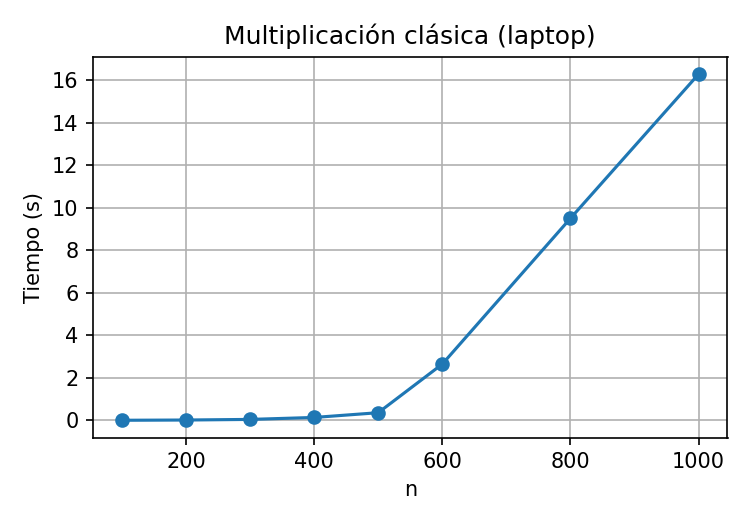
\includegraphics[width=0.48\textwidth]{../graficas/laptop_clasica.png}
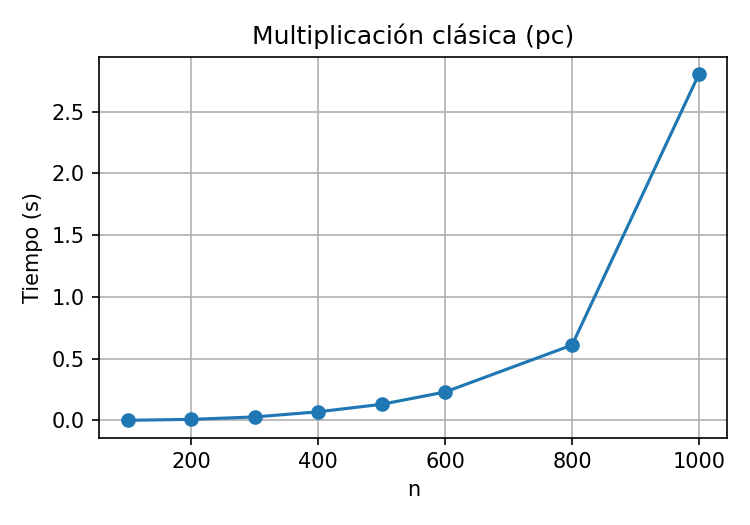
\includegraphics[width=0.48\textwidth]{../graficas/pc_clasica.png}
\caption{Tiempo de la multiplicación clásica en la laptop (izquierda) y en la PC (derecha).}
\label{fig:clasica}
\end{figure}

\subsection{Análisis}

Para tamaños pequeños el tiempo crece de forma parecida a $n^3$ y el tiempo
por operación se mantiene casi constante (1 a 3 ns). Pero a partir de cierto
tamaño el tiempo crece mucho más rápido que $n^3$:

\begin{itemize}
\item En la \textbf{laptop}, al pasar de $n=500$ a $n=600$ el tamaño aumenta
      solo 1,2 veces, pero el tiempo se multiplica por \textbf{7,4}
      (la teoría predice $1{,}2^3 \approx 1{,}73$). De $n=500$ a $n=1000$ el
      tiempo se multiplica por 45,5 en lugar de 8.
\item En la \textbf{PC} el salto aparece más tarde, entre $n=800$ y
      $n=1000$, donde el tiempo se multiplica por 4,6 (la teoría predice
      1,95). De $n=500$ a $n=1000$ se multiplica por 21,5.
\end{itemize}

El algoritmo sigue haciendo $n^3$ operaciones; lo que aumenta es el costo
de cada operación, porque cada vez más datos no están en la caché y hay que
traerlos de la memoria principal. El salto ocurre antes en la laptop porque
su caché L3 es 4 veces más pequeña.

La causa está en la línea interna: \texttt{A[i*n+k]} avanza de uno en uno
(recorre una fila de $A$, buen acceso), pero \texttt{B[k*n+j]} avanza de
$n$ en $n$ (recorre una columna de $B$), que es el mismo mal patrón del
segundo par de bucles de la sección anterior, pero repetido $n^2$ veces.

%------------------------------------------------------------
\section{Multiplicación de matrices por bloques}

\subsection{Fundamento}

La idea es dividir las matrices en submatrices (bloques) de tamaño
$b \times b$ y multiplicar bloque por bloque. El resultado es el mismo
porque el producto de matrices se puede hacer por partes:
\[
C_{IJ} = \sum_{K} A_{IK} \, B_{KJ}.
\]
La ventaja es que un bloque pequeño cabe completo en la caché, así que
mientras se trabaja con él casi todos los datos ya están cargados. Se
recorren los mismos elementos, pero ``por pedazos''.

\subsection{Código}

\begin{lstlisting}[caption={Multiplicación por bloques con seis bucles (\texttt{bloques.cpp}).}]
for (int ii = 0; ii < n; ii += b)
    for (int jj = 0; jj < n; jj += b)
        for (int kk = 0; kk < n; kk += b)
            for (int i = ii; i < min(ii + b, n); i++)
                for (int j = jj; j < min(jj + b, n); j++)
                    for (int k = kk; k < min(kk + b, n); k++)
                        C[i * n + j] += A[i * n + k] * B[k * n + j];
\end{lstlisting}

Los tres primeros bucles eligen el bloque y los tres últimos hacen la
multiplicación dentro del bloque. La función \texttt{min} sirve para que el
último bloque no se salga de la matriz cuando $n$ no es múltiplo de $b$.
Para verificar la implementación se usó el programa \texttt{verificar.cpp},
que compara elemento por elemento el resultado de la versión por bloques con
el de la clásica, usando matrices con valores distintos en cada posición. Se
eligió $n=500$ y $b=32$ porque 500 no es múltiplo de 32 y el último bloque
queda incompleto (20 filas), que es donde un error en el uso de \texttt{min}
se haría visible. Los dos resultados fueron idénticos.

\subsection{Complejidad}

Cada elemento $C_{ij}$ sigue recibiendo sus $n$ sumas, solo que en otro
orden. El número total de operaciones sigue siendo $n^3$, por lo que la
complejidad también es $O(n^3)$.

\subsection{Resultados}

Se probaron bloques de 16, 32, 64 y 128. El cuadro~\ref{tab:bloques}
muestra los tamaños más interesantes; entre paréntesis se indica cuántas
veces es más rápida que la clásica.

\begin{table}[H]
\centering
\caption{Tiempo (s) de la multiplicación por bloques y mejora respecto a la clásica.}
\label{tab:bloques}
\small
\begin{tabular}{llrrrrr}
\toprule
Equipo & $n$ & Clásica & $b=16$ & $b=32$ & $b=64$ & $b=128$ \\
\midrule
Laptop & 500  & 0,358  & 0,180 (2,0×) & 0,191 (1,9×) & 0,183 (2,0×) & 0,188 (1,9×) \\
Laptop & 800  & 9,509  & 1,112 (8,5×) & 1,155 (8,2×) & \textbf{0,888 (10,7×)} & 0,925 (10,3×) \\
Laptop & 1000 & 16,298 & 2,019 (8,1×) & \textbf{1,495 (10,9×)} & 1,522 (10,7×) & 1,738 (9,4×) \\
\midrule
PC & 500  & 0,130 & 0,110 (1,18×) & \textbf{0,108 (1,21×)} & 0,114 (1,14×) & 0,126 (1,03×) \\
PC & 800  & 0,610 & \textbf{0,500 (1,22×)} & 0,533 (1,14×) & 0,541 (1,13×) & 0,569 (1,07×) \\
PC & 1000 & 2,805 & 0,934 (3,00×) & \textbf{0,908 (3,09×)} & 0,960 (2,92×) & 1,033 (2,72×) \\
\bottomrule
\end{tabular}
\end{table}

\begin{figure}[H]
\centering
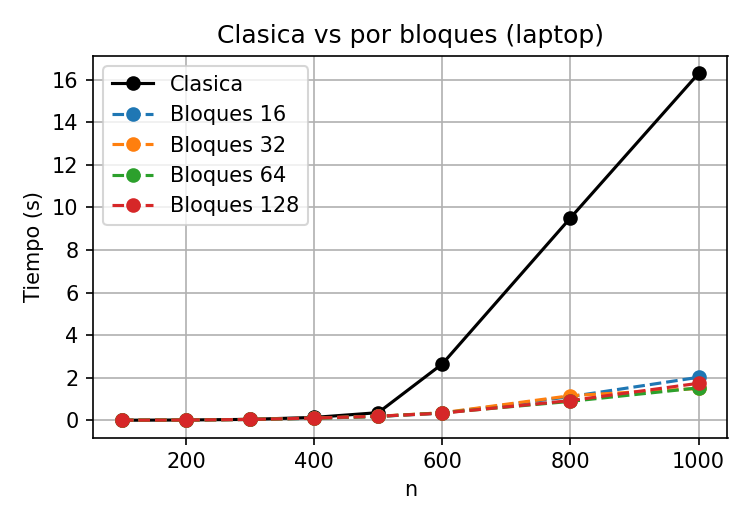
\includegraphics[width=0.48\textwidth]{../graficas/laptop_clasica_vs_bloques.png}
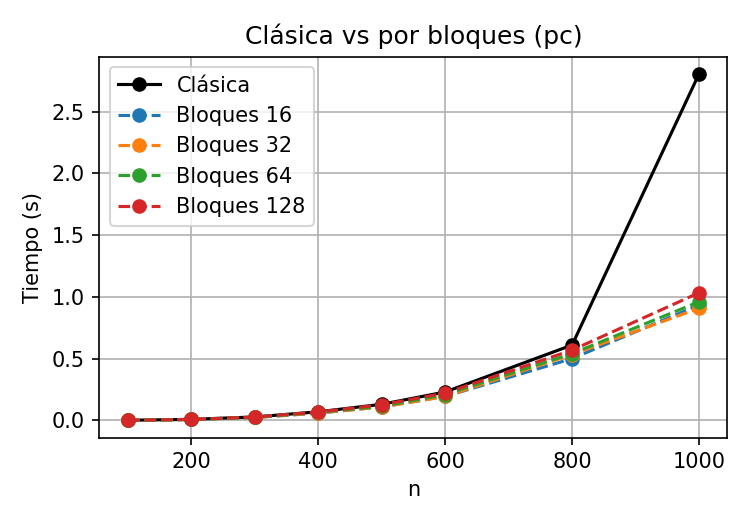
\includegraphics[width=0.48\textwidth]{../graficas/pc_clasica_vs_bloques.png}
\caption{Clásica frente a bloques en la laptop (izquierda) y en la PC (derecha).}
\label{fig:bloques}
\end{figure}

\begin{figure}[H]
\centering
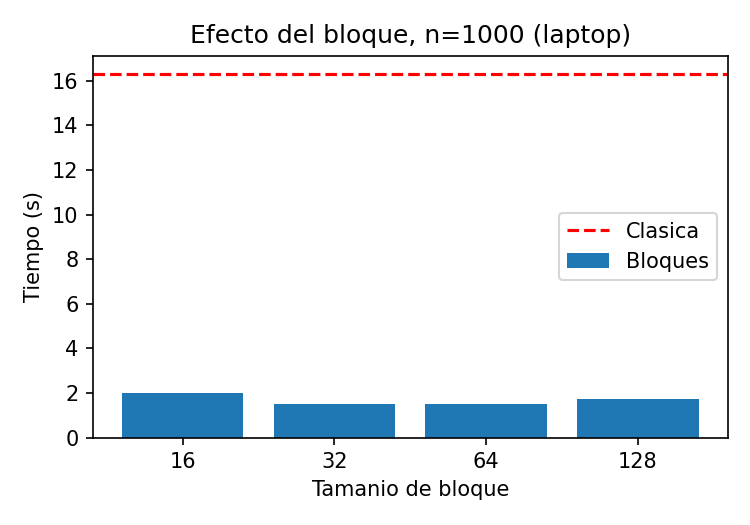
\includegraphics[width=0.48\textwidth]{../graficas/laptop_tam_bloque.png}
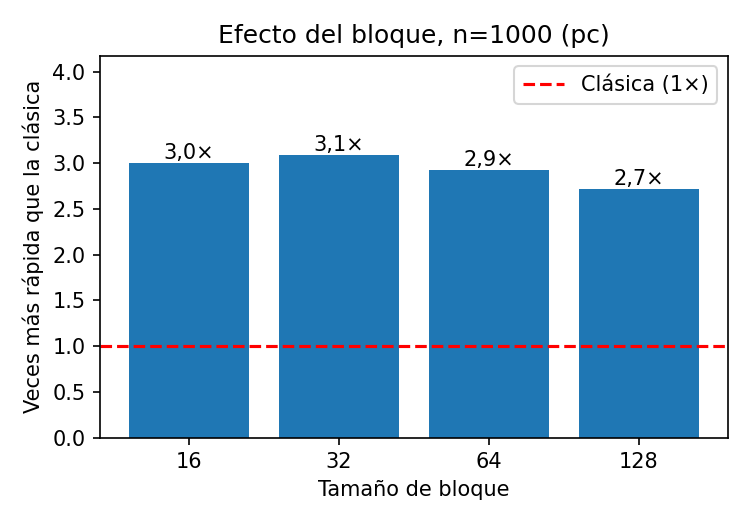
\includegraphics[width=0.48\textwidth]{../graficas/pc_tam_bloque.png}
\caption{Speedup de la multiplicación por bloques respecto a la clásica para
$n=1000$ (tiempo de la clásica dividido entre el tiempo con bloques), según el
tamaño de bloque. La línea roja (1×) representa la multiplicación clásica.}
\label{fig:tambloque}
\end{figure}

\subsection{Análisis}

\begin{itemize}
\item Para matrices pequeñas ($n \le 300$) casi no hay diferencia, porque las
      matrices completas ya caben en la caché.
\item Cuando las matrices dejan de caber, la versión por bloques es mucho más
      rápida: hasta \textbf{10,9 veces} en la laptop y \textbf{3,1 veces} en
      la PC para $n=1000$. La mejora es mayor en la laptop porque su caché L3
      es más pequeña y la versión clásica sufre más.
\item En la laptop, la versión por bloques con $n=1000$ tarda 1,5 s, mientras
      que la clásica tarda 16,3 s, aunque ambas hacen $10^9$ multiplicaciones.
\end{itemize}

\textbf{Tamaño de bloque.} Durante la multiplicación de un bloque se
necesitan tres bloques a la vez ($A$, $B$ y $C$). Para que quepan en la
caché L1 de 32 KB se debe cumplir
\[
3 \cdot b^2 \cdot 8 \text{ bytes} \le 32\,768 \quad\Rightarrow\quad b \le 36,
\]
por lo que se esperaba que $b=32$ fuera un buen valor. Los resultados lo
confirman: $b=32$ es el mejor para $n=1000$ en los dos equipos, aunque las
diferencias entre 16, 32 y 64 son pequeñas. Con $b=128$ los bloques ya no
caben en L1 y el tiempo empeora un poco. Con bloques muy pequeños también
se pierde algo, probablemente por el costo de controlar los seis bucles.

\textbf{¿Por qué es más rápida si la complejidad es la misma?} Porque la
complejidad solo cuenta operaciones. La versión por bloques hace las mismas
operaciones, pero ordenadas para que los datos que necesita estén casi
siempre en la caché. Esto se comprueba con Cachegrind en la
sección~\ref{sec:valgrind}.

%------------------------------------------------------------
\section{Movimiento de datos y memoria caché}

\subsection{Localidad espacial y temporal}

\begin{itemize}
\item \textbf{Localidad espacial:} si un programa usa un dato, es probable que
      use pronto los datos que están a su lado. Por eso la caché no carga un
      solo dato, sino una línea de 64 bytes (8 valores \texttt{double}).
\item \textbf{Localidad temporal:} si un programa usa un dato, es probable que
      lo vuelva a usar pronto. Por eso la caché guarda los datos usados
      recientemente.
\end{itemize}

\subsection{Cómo se accede a las matrices}

\begin{table}[H]
\centering
\caption{Patrón de acceso en el bucle más interno.}
\label{tab:patron}
\begin{tabular}{lll}
\toprule
Acceso & Clásica & Bloques \\
\midrule
\texttt{A[i*n+k]} & avanza de 1 en 1 (fila) & avanza de 1 en 1, solo $b$ elementos \\
\texttt{B[k*n+j]} & salta $n$ posiciones (columna) & salta $n$ posiciones, solo $b$ elementos \\
\texttt{C[i*n+j]} & fijo durante el bucle & fijo durante el bucle \\
\bottomrule
\end{tabular}
\end{table}

En la \textbf{clásica}, para calcular un solo elemento de $C$ se recorre una
columna entera de $B$ ($n$ elementos, cada uno en una línea de caché
distinta). Cuando se pasa al siguiente $j$, se recorre otra columna completa.
Los datos de $B$ se vuelven a usar (hay localidad temporal), pero pasa
tanto tiempo entre un uso y otro que la caché ya los ha descartado.

En la de \textbf{bloques}, el recorrido de $B$ sigue saltando de $n$ en $n$,
pero solo $b$ elementos seguidos. Esos $b$ elementos caben en la caché y se
reutilizan muchas veces antes de pasar al siguiente bloque. Es decir, el
bloqueo aprovecha mejor la localidad temporal.

\subsection{Complejidad y costo del movimiento de datos}

El tiempo real se puede ver como la suma de dos partes:
\[
t \approx (\text{operaciones}) \times t_{\text{op}} + (\text{fallos de caché}) \times t_{\text{fallo}}.
\]
La primera parte es la que mide la complejidad y es igual en ambas
versiones. La segunda depende de cómo se accede a la memoria. Como traer un
dato de memoria principal cuesta mucho más que una suma o una
multiplicación, cuando hay muchos fallos la segunda parte domina. Esto es
lo que se ve en el cuadro~\ref{tab:clasica}: el tiempo por operación pasa de
unos 2 ns a más de 16 ns en la laptop cuando las matrices dejan de caber en
la caché.

%------------------------------------------------------------
\section{Evaluación con Valgrind y KCachegrind}
\label{sec:valgrind}

\subsection{Configuración}

Se usó Cachegrind indicando los tamaños reales de caché de cada equipo:

\begin{lstlisting}[language=bash,numbers=none,caption={Comandos usados (\texttt{cachegrind.sh}).}]
# Laptop (L3 = 3 MB)
valgrind --tool=cachegrind --I1=32768,8,64 --D1=32768,8,64 \
         --LL=3145728,12,64 ./clasica 512
# PC (L3 = 12 MB)
valgrind --tool=cachegrind --I1=32768,8,64 --D1=32768,8,64 \
         --LL=12582912,12,64 ./clasica 512
\end{lstlisting}

Cachegrind simula dos niveles: el primer nivel (I1 para instrucciones y D1
para datos) y el último nivel (LL, que corresponde a L3). No simula L2.
Para la L3 de la PC se usó asociatividad 12 en lugar de 16, porque
Cachegrind exige que el número de conjuntos sea potencia de 2; el tamaño
de 12 MB se mantuvo. Si no se indican los parámetros, Valgrind hace un ajuste
equivalente por su cuenta y usa 24 vías; en ambos casos se conserva la
capacidad, que es lo que determina si las matrices caben en el último nivel.
Todos los resultados de este informe se obtuvieron con la configuración de
12 vías.

\subsection{Resultados con $n=512$}

Los contadores de instrucciones, accesos y fallos de D1 salieron
prácticamente idénticos en los dos equipos, porque tienen la misma caché L1.
Solo cambian los fallos del último nivel (LLd).

\begin{table}[H]
\centering
\caption{Cachegrind con $n=512$ y bloque $b=32$.}
\label{tab:cg512}
\begin{tabular}{lrr}
\toprule
Contador & Clásica & Bloques ($b=32$) \\
\midrule
Instrucciones ejecutadas (I refs) & 1\,083\,487\,547 & 1\,155\,845\,875 \\
Fallos caché de instrucciones (I1) & 1\,776 & 1\,795 \\
Accesos a datos (D refs) & 406\,222\,953 & 441\,466\,510 \\
Fallos caché de datos D1 & 134\,761\,071 & 136\,098\,896 \\
Tasa de fallos D1 & 33,2\,\% & 30,8\,\% \\
Fallos último nivel LLd (laptop) & 252\,907 & 256\,886 \\
Fallos último nivel LLd (PC) & 104\,713 & 104\,715 \\
\bottomrule
\end{tabular}
\end{table}

Este resultado fue inesperado: con $n=512$ la versión por bloques
\textbf{casi no reduce} los fallos de D1 (de 33,2\,\% a 30,8\,\%).

\subsection{Prueba adicional con $n=500$}

La sospecha fue que el problema era usar un tamaño potencia de 2. La caché
D1 tiene $32\,768 / (64 \cdot 8) = 64$ conjuntos y 8 vías. Con $n=512$, dos
elementos seguidos de una columna de $B$ están separados $8 \cdot 512 = 4096$
bytes, es decir exactamente 64 líneas. Como $64$ es múltiplo del número de
conjuntos, \textbf{todos los elementos de la columna caen en el mismo
conjunto}, y ese conjunto solo puede guardar 8 líneas. Por eso, aunque el
bloque de 32 elementos cabe en L1 por tamaño, se siguen expulsando datos
entre sí.

Para comprobarlo se repitió la prueba con $n=500$, donde la separación es
de 4000 bytes (62,5 líneas) y los elementos se reparten entre conjuntos
distintos:

\begin{table}[H]
\centering
\caption{Cachegrind con $n=500$ frente a $n=512$.}
\label{tab:cg500}
\begin{tabular}{lrrr}
\toprule
Caso & I refs & Fallos D1 & Tasa D1 \\
\midrule
Clásica, $n=500$ & 1\,009\,405\,597 & 113\,082\,929 & 29,9\,\% \\
Bloques $b=32$, $n=500$ & 1\,078\,492\,459 & \textbf{1\,866\,176} & \textbf{0,5\,\%} \\
\midrule
Clásica, $n=512$ & 1\,083\,487\,547 & 134\,761\,071 & 33,2\,\% \\
Bloques $b=32$, $n=512$ & 1\,155\,845\,875 & 136\,098\,896 & 30,8\,\% \\
Bloques $b=8$, $n=512$ & 1\,427\,731\,852 & 139\,579\,509 & 24,0\,\% \\
\bottomrule
\end{tabular}
\end{table}

Con $n=500$ la versión por bloques tiene \textbf{60 veces menos fallos} de
D1 que la clásica (1,9 millones frente a 113 millones). Esto confirma que el
bloqueo sí reduce los fallos de caché, pero con $n=512$ el conflicto de
asociatividad lo impide. Incluso con bloques de 8 la tasa sigue en 24\,\%,
probablemente porque las 8 vías del conjunto también las ocupan las líneas
de $A$ y $C$.

\subsection{Análisis}

\begin{enumerate}
\item \textbf{Instrucciones ejecutadas:} la versión por bloques ejecuta
      \emph{más} instrucciones que la clásica (6,8\,\% más con $n=500$),
      porque tiene tres bucles extra y las comparaciones con \texttt{min}. Aun así
      es más rápida. El número de instrucciones no explica el tiempo.
\item \textbf{Accesos a memoria:} son del mismo orden en las dos versiones
      (unos 400 millones), porque leen los mismos datos.
\item \textbf{Fallos en la caché de datos:} aquí está la diferencia. En la
      clásica, casi 1 de cada 3 accesos a datos falla en D1. En la de
      bloques con $n=500$ falla menos de 1 de cada 200.
\item \textbf{Fallos en la caché de instrucciones:} son despreciables (menos
      de 2\,000 en más de mil millones de instrucciones). El código de los
      bucles es pequeño y cabe entero en I1, así que el problema está en los
      datos y no en el código.
\item \textbf{Último nivel (LL):} la laptop tiene más del doble de fallos LLd
      que la PC (253 mil frente a 105 mil), porque su L3 es 4 veces más
      pequeña. Con $n=512$ las tres matrices ocupan 6 MB: no caben en los
      3 MB de la laptop, pero sí en los 12 MB de la PC.
\end{enumerate}

\subsection{KCachegrind}

Los archivos \texttt{.out} generados se abrieron con KCachegrind:

\begin{lstlisting}[language=bash,numbers=none]
kcachegrind cachegrind/extra_clasica_500.out
kcachegrind cachegrind/extra_bloques_500_32.out
kcachegrind cachegrind/clasica_512.out
\end{lstlisting}

En cada uno se seleccionó el evento \texttt{L1 Data Read Miss} (D1mr, fallos
de lectura en D1), la función \texttt{main} y la pestaña \texttt{Source Code},
que muestra los fallos atribuidos a cada línea del código. Lo mismo se
obtiene en texto con \texttt{cg\_annotate}.

\begin{figure}[H]
\centering
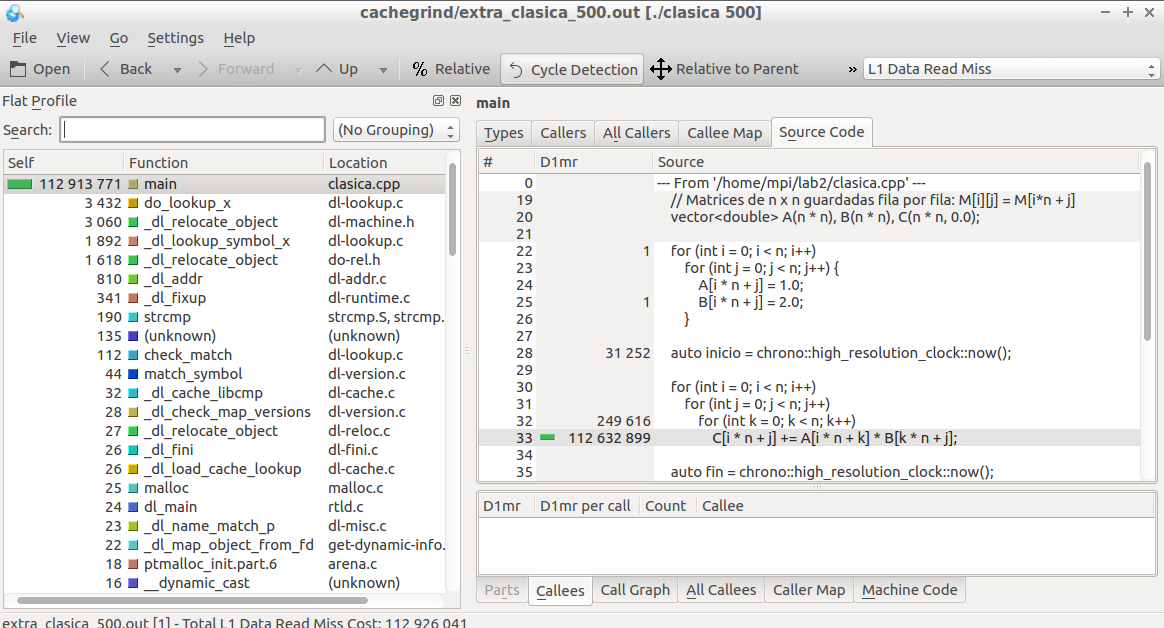
\includegraphics[width=\textwidth]{../graficas/kcachegrind_clasica_500.png}
\caption{KCachegrind, multiplicación clásica ($n=500$), evento D1mr: la línea
33 tiene 112\,632\,899 fallos de lectura en D1.}
\label{fig:kcachegrind500c}
\end{figure}

\begin{figure}[H]
\centering
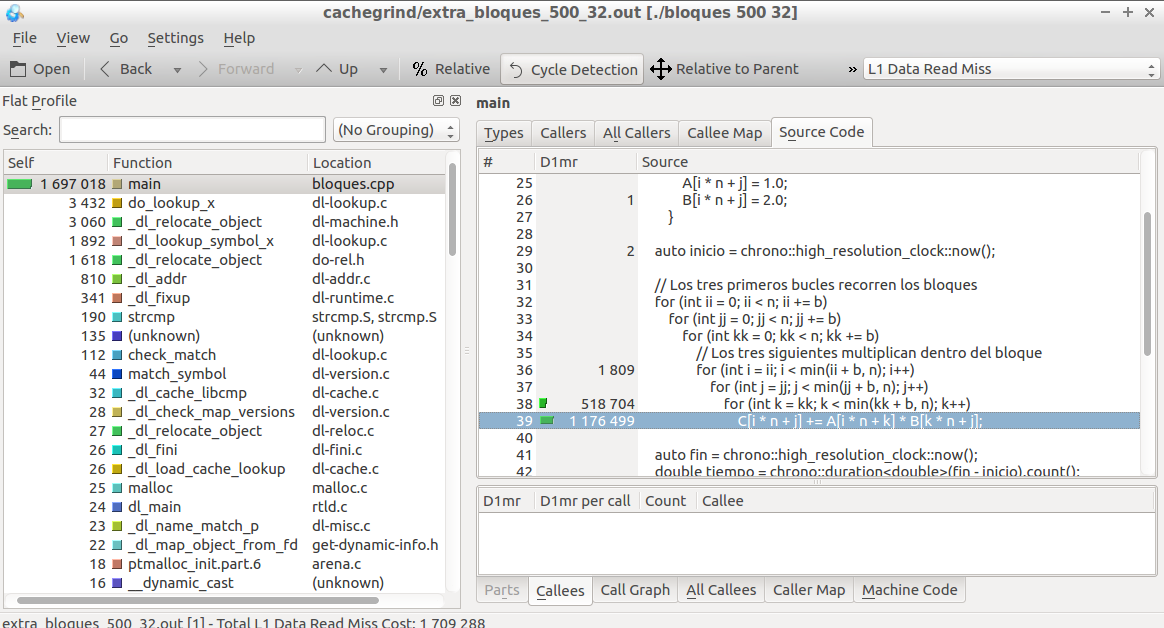
\includegraphics[width=\textwidth]{../graficas/kcachegrind_bloques_500.png}
\caption{KCachegrind, multiplicación por bloques ($n=500$, $b=32$), evento
D1mr: la misma operación (línea 39) tiene 1\,176\,499 fallos.}
\label{fig:kcachegrind500b}
\end{figure}

Con $n=500$, la línea de la multiplicación de la versión clásica tiene
\textbf{112\,632\,899} fallos de lectura en D1, el \textbf{99,7\,\%} del total
del programa (112\,926\,041). En la versión por bloques, la misma operación
tiene solo \textbf{1\,176\,499}, unas \textbf{96 veces menos}.
También se revisó el evento \texttt{LL Data Read Miss} (DLmr, fallos de
lectura en el último nivel) para la clásica con $n=500$ en los dos equipos
(figuras~\ref{fig:kcachegrindlll} y~\ref{fig:kcachegrindllp}). Las tres
matrices ocupan unos 5,7 MB: no caben en la L3 de 3 MB de la laptop, donde la
línea de la multiplicación produce 39\,972 fallos (77\,770 en todo el
programa), pero sí caben en la L3 de 12 MB de la PC, donde \texttt{main} tiene
un único fallo, en la inicialización, y la multiplicación no tiene ninguno
(6\,038 en todo el programa, casi todos de la carga de bibliotecas). En los
dos equipos la misma línea tiene 112,6 millones de fallos en D1, de modo que
casi todos esos fallos se resuelven antes de llegar a la memoria principal.

\begin{figure}[H]
\centering
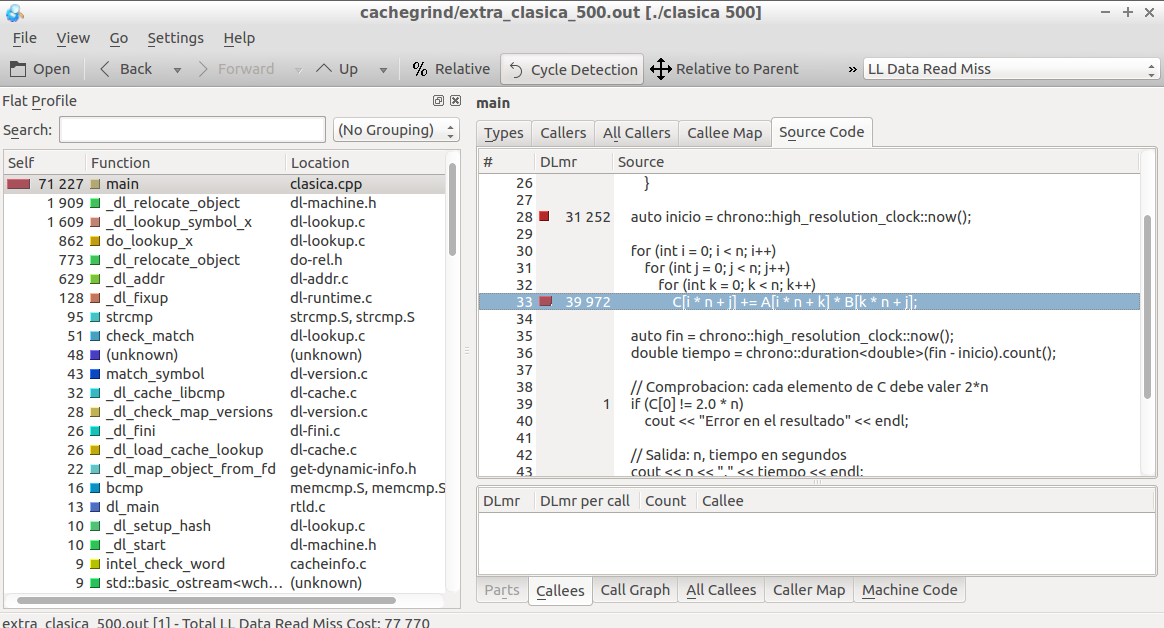
\includegraphics[width=\textwidth]{../graficas/kcachegrind_ll_laptop.png}
\caption{KCachegrind, laptop (L3 de 3 MB), clásica $n=500$, evento DLmr: la
línea 33 tiene 39\,972 fallos de lectura en el último nivel.}
\label{fig:kcachegrindlll}
\end{figure}

\begin{figure}[H]
\centering
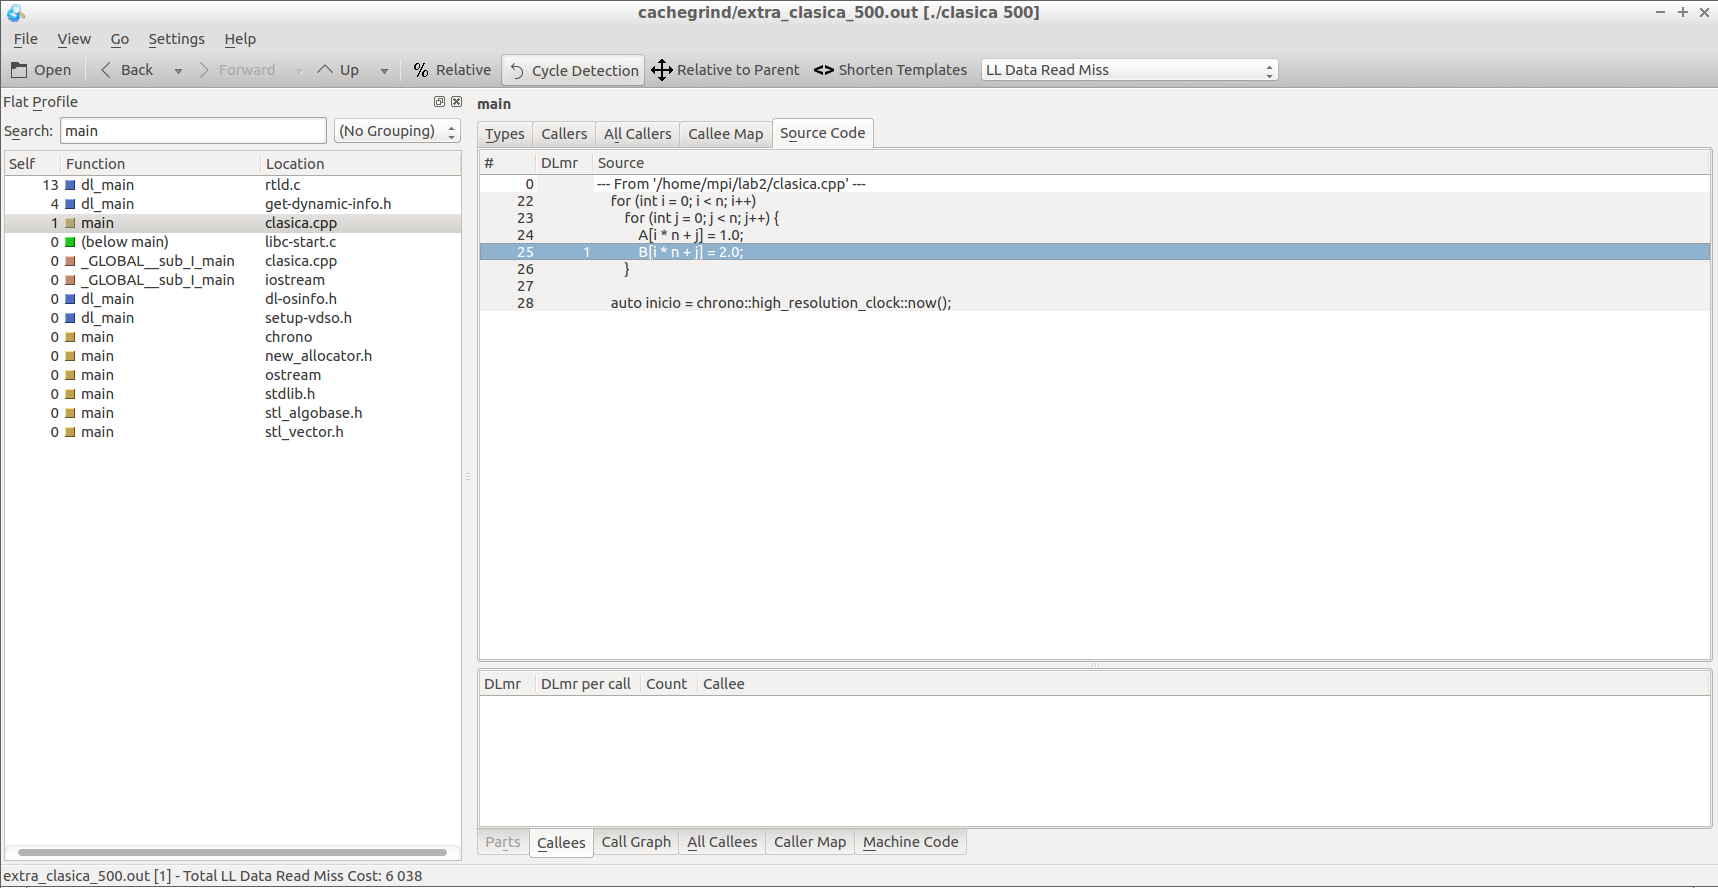
\includegraphics[width=\textwidth]{../graficas/kcachegrind_ll_pc.png}
\caption{KCachegrind, PC (L3 de 12 MB), clásica $n=500$, evento DLmr:
\texttt{main} tiene un solo fallo (línea 25, inicialización) y la línea de la
multiplicación ninguno.}
\label{fig:kcachegrindllp}
\end{figure}

\begin{figure}[H]
\centering
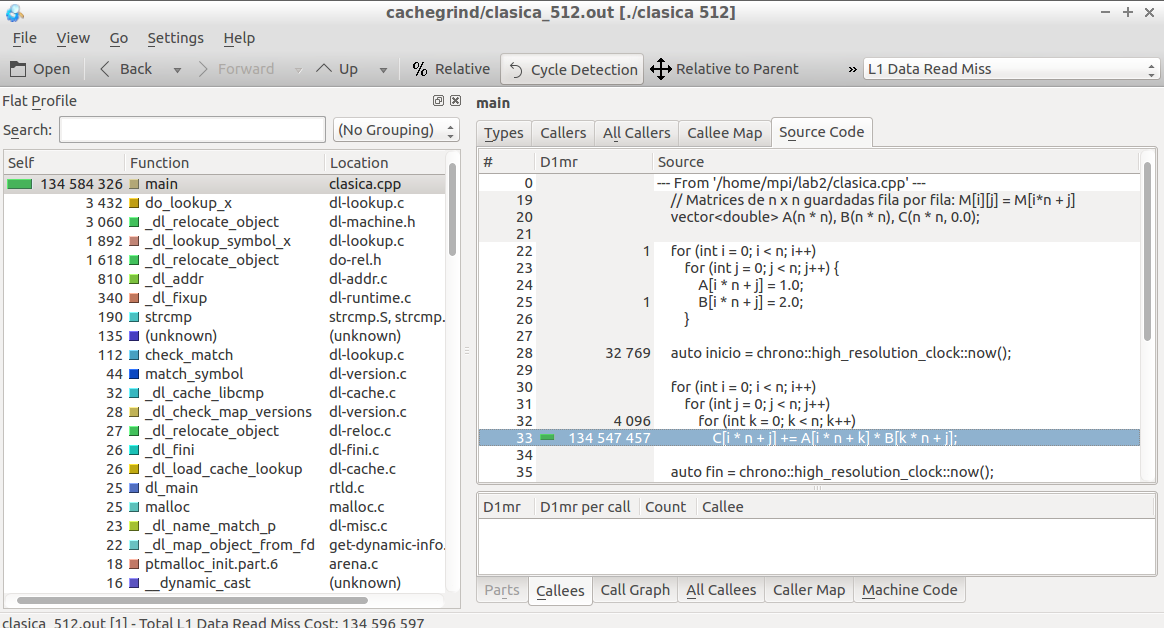
\includegraphics[width=\textwidth]{../graficas/kcachegrind.png}
\caption{KCachegrind, multiplicación clásica ($n=512$): la línea 33 tiene
134\,547\,457 fallos de lectura en D1, el 99,96\,\% del total (134\,596\,597).}
\label{fig:kcachegrind512}
\end{figure}

%------------------------------------------------------------
\section{Conclusiones}

\begin{enumerate}
\item Los dos pares de bucles de Pacheco hacen las mismas $\mathit{MAX}^2$ iteraciones,
      pero recorrer la matriz por columnas fue hasta 20 veces más lento en la
      laptop y 8,7 veces en la PC. La única diferencia es el orden de acceso
      a la memoria.
\item La multiplicación clásica es $O(n^3)$, pero cuando las matrices dejan de
      caber en la caché el tiempo crece mucho más rápido que $n^3$: en la
      laptop, de $n=500$ a $n=1000$ el tiempo se multiplicó por 45 en lugar
      de 8.
\item La multiplicación por bloques tiene la misma complejidad, pero fue hasta
      10,9 veces más rápida en la laptop y 3,1 veces en la PC. El mejor tamaño
      de bloque fue cercano a 32, como se esperaba por el tamaño de L1.
\item Cachegrind mostró que la diferencia no está en el número de
      instrucciones (la versión por bloques ejecuta más), sino en los fallos
      de caché de datos: con $n=500$ bajaron de 113 millones a 1,9 millones.
\item Se encontró que con $n=512$ el bloqueo casi no reduce los fallos de D1,
      por un conflicto de asociatividad de la caché. Usar tamaños potencia
      de 2 puede ocultar el beneficio del bloqueo.
\item El equipo con caché más pequeña (la laptop) es el que más se beneficia
      de escribir código que respete la localidad.
\end{enumerate}

%------------------------------------------------------------
\section{Repositorio}

El código fuente, los scripts, los resultados en CSV y las instrucciones de
compilación están en:

\begin{center}
\url{https://github.com/dtamotu/Lab2-Evaluacion-desempeno-algoritmos-memoria-cache}
\end{center}

%------------------------------------------------------------
\begin{thebibliography}{9}
\bibitem{pacheco}
P. S. Pacheco, \emph{An Introduction to Parallel Programming}. Morgan Kaufmann, 2011.

\bibitem{hennessy}
J. L. Hennessy y D. A. Patterson, \emph{Computer Architecture: A Quantitative Approach}, 6.\textsuperscript{a} ed. Morgan Kaufmann, 2017.

\bibitem{valgrind}
Valgrind Developers, ``Cachegrind: a high-precision tracing profiler'',
\url{https://valgrind.org/docs/manual/cg-manual.html}.
\end{thebibliography}

\end{document}
